\chapter{Ausarbeitung}
\section{a}
There are 110 heads in 200 tosses, the frequency is 55\%, which means it is possible that the coin is unfair.
\section{b}
Bayes'theorem:
\begin{equation*}
	prob(H|\{results\}) = \frac{prob(\{results\}|H) prob(H)}{prob(\{results\})}
\end{equation*}
\begin{itemize}
	\item likelihood func: $prob(\{results\}|H)$
	\item prior func: $prob(H)$
\end{itemize}
\section{c}
Münzenwurf gehört zur Binomialverteilung.
\begin{equation*}
	prob(\{results\}|H) = \begin{bmatrix}
		N \\
		R
	\end{bmatrix} \cdot H^R (1-H)^(N-R) = \frac{N!}{R!(N-R)!}H^R(1-H)^{(N-R)}
\end{equation*}
\section{d \& e}
The posterior pdf is in \autoref{fig:pdf}. because the first tosses are head, so when N = 1~3, the maximum value of pdf is when $H = 1$. The fourth toss is, so the pdf returns 0 for $H = 1$, the max pdf ist at $H = 0.75$. When we have 200 tosses, there is more possibility, the maximal value is at $H = 0.55$.
\begin{figure}[htpb]\centering
	\subfigure[pdf]{
		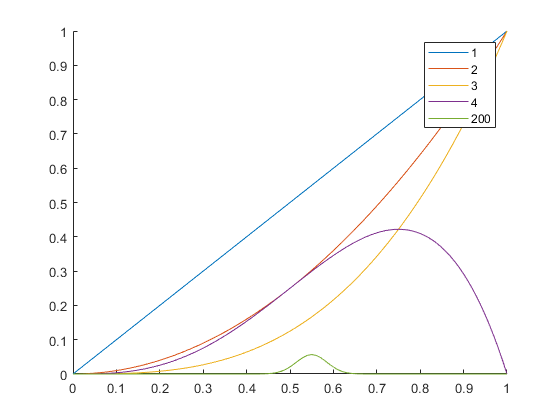
\includegraphics[width=0.9\textwidth]{1.png}}
	\caption{PDF}
	\label{fig:pdf}
\end{figure}\\
\section{f}
\begin{gather*}
	P_{N} = \frac{\frac{N!}{R!(N-R)!}H^R(1-H)^{(N-R)} \cdot prob(H)}{prob(\{results\})} \\
	P_{N+1} = \frac{\frac{(N+1)!}{(R)!(N+1-R)!}H^{R}(1-H)^{(N+1-R)} \cdot prob(H)}{prob(\{results\})} \\
	\frac{P_{N+1}}{P_{N}} = \frac{(N+1)(1-H)}{N+1-R}(1-H) \\
	P_{N+1} = \frac{(N+1)(1-H)}{N+1-R}(1-H) \cdot P_{N}
\end{gather*}
\section{g}
\begin{figure}[htpb]\centering
	\subfigure[]{
		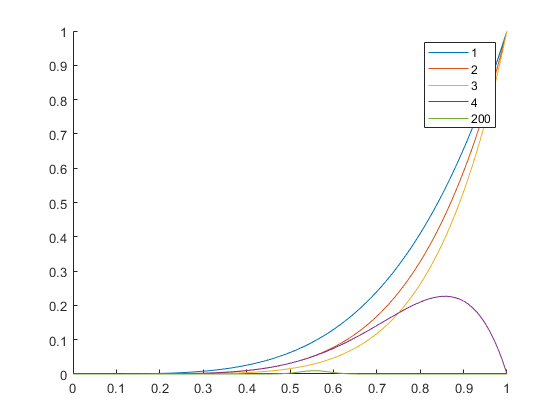
\includegraphics[width=0.9\textwidth]{2.png}}
	\caption{$3H^2$}
	\label{fig:pdf2}
\end{figure}
\begin{figure}[htpb]\centering
	\subfigure[]{
		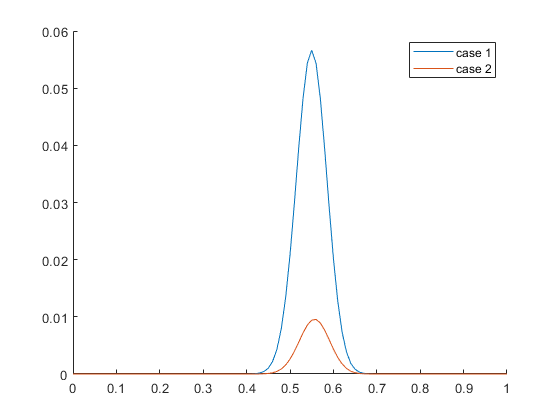
\includegraphics[width=0.9\textwidth]{3.png}}
	\caption{N = 200}
	\label{fig:pdf3}
\end{figure}
In this case, the coin is tend to be more unfair compared to (e) \autoref{fig:pdf2}, the height of the peak is also lower\autoref{fig:pdf3}. (This distribution is not exactly correct because of the accuracy limit of Matlab).
\clearpage
\section{Maximum-Liklihood-Methode}
\begin{equation*}
	prob(\{results\}|H) =  \frac{N!}{R!(N-R)!}H^R(1-H)^{(N-R)}
\end{equation*}
\begin{align*}
	\log\mathcal{L}(H) =& \log\frac{N!}{R!(N-R)!} + \log H^R + \log (1-H)^{(N-R)} \\
	=& R \log H + (N-R) \log (1-H) \\
\end{align*}
Um die maximale Werte zu berechnen:
\begin{gather*}
	\frac{\partial \log\mathcal{L}(H)}{\partial H} = R\cdot \frac{1}{H} - (N-R)\frac{1}{1-H} = \frac{R-HN}{H(1-H)} \\
\end{gather*}
When $R = HN$, also $H = \frac{R}{N}$, Likelihood function is maximum.